\chapter{Building Blocks of CNNs}\label{chp:3}
To understand how CNNs work, it’s crucial to break down their architecture into core components. These blocks — \textbf{Convolutional Layers}, \textbf{Pooling Layers}, \textbf{Activation Functions}, \textbf{Fully Connected Layers}, and \textbf{Dropout Layers} — work together to extract and classify patterns in data.\\

\begin{figure}[h!]
    \centering
    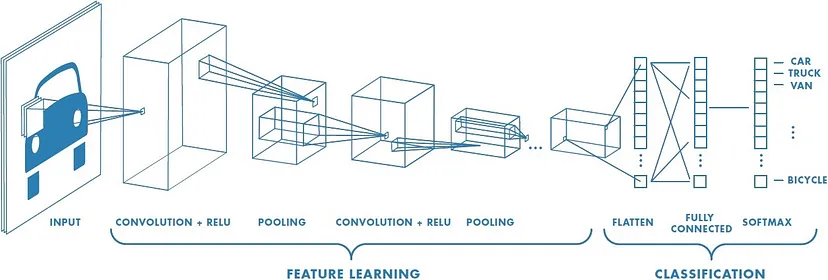
\includegraphics[width=\textwidth]{images/figure4.png}
    \caption{A typical Convolutional Neural Network architecture}
    \label{fig:4}
\end{figure}

An input image can usually be represented as a matrix with corresponding pixel values. It can have multiple such matrices depending on the number of color channels of the input image.

\begin{figure}[h!]
    \centering
    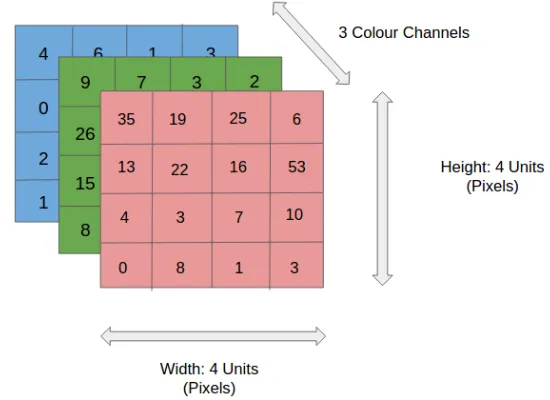
\includegraphics[width=0.5\textwidth]{images/figure5.png}
    \caption{A sample $4 \times 4 \times 3$ RGB input image}
    \label{fig:5}
\end{figure}

In figure \ref{fig:5}, we have an RGB image that has been separated by its three color planes — Red, Green, and Blue. There are a number of such color spaces in which images exist — Grayscale, RGB, HSV, CMYK, etc.\\

You can imagine how computationally intensive things would get once the images reach dimensions, say 8K ($7680 \times 4320$). The primary function of a ConvNet is to transform images into a more manageable representation while preserving the essential features needed for accurate predictions. This is crucial when designing an architecture that is good at feature extraction as well as remains scalable to large datasets.

\section{Convolutional Layers: The Core Component}
The convolutional layer is the most fundamental building block of CNNs. It is responsible for detecting spatial features (e.g., edges, textures) by applying a \textbf{kernel} or \textbf{filter} to the input data.

\subsection{How Convolution Works}
Convolution is the heart of CNNs. It is a mathematical operation where a filter slides (or convolves) over the input matrix to compute a feature map. In other words, the filter or kernel is applied to the input image to compute feature maps. The operation captures local patterns, which are then combined to form higher-level patterns.\\

\begin{figure}
    \centering
    % \includegraphics{}
     \animategraphics[width=0.5\textwidth, loop, autoplay]{1} %frame rate
    {images/figure6/figure6-} %path to figures
    {0} %start index
    {8} %end index
    \caption{Convolving a $5 \times5 \times1$ image with a $3 \times3 \times1$ kernel to get a $3 \times3 \times1$ convolved feature}
    \label{fig:6}
\end{figure}

In figure \ref{fig:6}, a kernel (filter matrix) of size $3 \times 3$ slides over the input matrix (image) of size $5 \times 5$ to produce an output feature map (convolved feature) of size $3 \times 3$.\\

In general, any image matrix can be represented as Height $\times$ Width $\times$ No. of channels. In figure \ref{fig:6}, no. of channels is considered as $1$.  For an input image matrix of size $W_{in} \times H_{in}$, the corresponding dimension of the output feature map (convolved feature) after convolving with a square kernel of dimension $k$ can be formularized as below:

\begin{equation}
    W_{out} = W_{in} - k +1
    \label{eqn:1}
\end{equation}

\begin{equation}
    H_{out} = H_{in} - k +1
    \label{eqn:2}
\end{equation}

In figure \ref{fig:6}, the green section resembles our $5 \times 5 \times 1$ input image, $I$. The kernel/filter, $K$, represented in color yellow, is selected as a $3 \times 3 \times 1$ matrix:\\

K = $\begin{bmatrix} 1 & 1 & 1\\ 0 & 1 & 1\\ 0 & 0 & 1\end{bmatrix}$.


\subsection{Is Kernel Always a Square Matrix?}
The kernel in a Convolutional Neural Network (CNN) does not always have to be square. Although square kernels (e.g., $3 \times 3$, $5 \times 5$) are the most commonly used due to their simplicity and symmetry, kernels can also have rectangular or non-square shapes depending on the application:
\begin{itemize}
    \item \textbf{Rectangular Kernels}:
    \begin{itemize}
        \item $3 \times 5$: Used when more detailed feature extraction is needed in one dimension (e.g., in text or speech recognition).
        \item $1 \times n$ or $n \times 1$: Common in 1D convolutions or when processing time-series data or text.
    \end{itemize}
    \item \textbf{Horizontal/Vertical Feature Extraction}:
    \begin{itemize}
        \item A $1 \times 3$ kernel emphasizes horizontal patterns, while a $3 \times 1$ kernel highlights vertical patterns.
    \end{itemize}
    \item \textbf{Custom Shapes}:
    \begin{itemize}
        \item For specialized use cases like detecting specific geometric patterns in images or reducing computational complexity in one dimension.
    \end{itemize}
\end{itemize}

\subsection{Stride and Padding}
In figure \ref{fig:6}, the kernel shifts 9 times, every time performing an element-wise multiplication operation (\textbf{Hadamard Product}) between kernel $K$ and the portion $P$ of the image matrix $I$ over which the kernel is hovering.\\

\begin{figure}[h!]
    \centering
    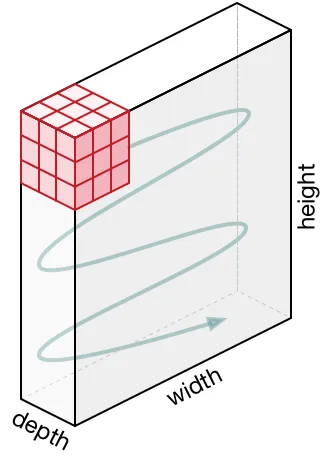
\includegraphics[width=0.2\textwidth]{images/figure7.png}
    \caption{Typical movement of a kernel matrix during convolution}
    \label{fig:7}
\end{figure}

Figure \ref{fig:7} shows the typical movement of a kernel matrix. The filter moves to the right with a certain \textbf{Stride Length} until it parses the complete width. Moving on, it hops down to the beginning (left) of the image with the same Stride Length and repeats the process until the entire image is traversed.\\

\begin{figure}
    \centering
    % \includegraphics{}
     \animategraphics[width=\textwidth, loop, autoplay]{1} %frame rate
    {images/figure8/figure8-} %path to figures
    {0} %start index
    {7} %end index
    \caption{Convolution operation on a $M \times N \times 3$ image matrix with a $3 \times 3 \times 3$ Kernel}
    \label{fig:8}
\end{figure}

As we can see in figure \ref{fig:8}, in the case of images with multiple channels (e.g. RGB), the Kernel has the same depth as that of the input image. Matrix Multiplication is performed between $K_n$ and $I_n$ stack ([$K_1$, $I_1$]; [$K_2$, $I_2$]; [$K_3$, $I_3$]) and all the results are summed with the bias to give us a squashed one-depth channel Convoluted Feature Output.\\

The number of shifts of the kernel depends on \textbf{stride length}. In our example in figure \ref{fig:6} and figure \ref{fig:8}, $\text{stride length} = 1$, which can also be called \textbf{non-strided}. Stride length denotes how many cells the kernel will skip before the next element-wise multiplication operation. Figure \ref{fig:9} shows a convolution operation with $\text{stride length} = 2$.\\

\begin{figure}
    \centering
    % \includegraphics{}
     \animategraphics[width=0.35\textwidth, loop, autoplay]{1} %frame rate
    {images/figure9/figure9-} %path to figures
    {0} %start index
    {8} %end index
    \caption{Convolution operation with $\text{stride length} = 2$}
    \label{fig:9}
\end{figure}

There are two types of results to the convolution operation — one in which the convolved feature is reduced in dimensionality as compared to the input (as explained by \ref{eqn:1} and \ref{eqn:2}), and the other in which the dimensionality is either increased or remains the same. This is done by applying \textbf{Valid Padding} in the case of the former, or \textbf{Same Padding} in the case of the latter.\\

\begin{figure}
    \centering
    % \includegraphics{}
     \animategraphics[width=0.4\textwidth, loop, autoplay]{1} %frame rate
    {images/figure10/figure10-} %path to figures
    {0} %start index
    {24} %end index
    \caption{Same padding - $5 \times 5 \times 1$ image is padded with $0$s to create a $6 \times 6 \times 1$ image}
    \label{fig:10}
\end{figure}

When we augment the $5 \times 5 \times 1$ image into a $6 \times 6 \times 1$ image by applying a $0$-vector at each end (\textbf{zero-padding}) and then apply the $3 \times 3 \times 1$ kernel over it, we find that the convolved matrix turns out to be of dimensions $5 \times 5 \times 1$. Hence the name — \textbf{Same Padding}.\\

On the other hand, if we perform the same operation without padding, we are presented with a matrix that has dimensions of the Kernel ($3 \times 3 \times 1$) itself — this is \textbf{Valid Padding}.\\

Considering stride length and padding, the dimension of the output feature map (convolved feature) after convolving an input image matrix of size $W_{in} \times H_{in}$ with a square kernel of dimension $k$, will be:

\begin{equation}
    W_{out} = \frac{W_{in} - k + 2P}{S} +1
    \label{eqn:3}
\end{equation}

\begin{equation}
    H_{out} = \frac{H_{in} - k + 2P}{S} +1
    \label{eqn:4}
\end{equation}

where, $W_{in}$ and $H_{in}$ are the dimensions of the input image, $W_{out}$ and $H_{out}$ are the dimensions of the convolved feature matrix, $k$ is the kernel size, $P$ is the padding size (amount of zero-padding applied to the input), and $S$ is the stride length of the convolution operation.

\subsection{Importance of Stride and Padding}
Stride and padding are crucial parameters in convolutional neural networks (CNNs) as they impact the output size, feature extraction, and computational efficiency.
\begin{itemize}
    \item \textbf{Stride determines the step size of the convolutional filter}; a stride of 1 is used when fine-grained feature extraction and preserving spatial details are important, while larger strides (e.g., 2) are employed to reduce the spatial dimensions and computational load.
    \item Padding involves adding extra pixels (typically zeros) around the input to \textbf{control the spatial size of the output}. "Same" padding is used when maintaining the input size is desired, while "valid" padding is chosen to avoid adding any extra pixels, resulting in smaller outputs.
\end{itemize}
Selecting appropriate stride and padding values depends on the task: for applications like object detection, smaller strides and "same" padding help retain spatial details, whereas larger strides and "valid" padding may be preferred for classification tasks requiring reduced spatial dimensions.\\

In summary, the purpose of the convolution operation is to \textbf{extract high-level features}, such as edges, from the input image. Convolutional Neural Networks (ConvNets) are not restricted to a single convolutional layer. Typically, the initial convolutional layer focuses on capturing low-level features like edges, colors, and gradient orientations. As additional layers are added, the network progressively adapts to detect high-level features, ultimately creating an architecture capable of comprehensively understanding the images in the dataset, much like humans do.\\

\subsection{Key Characteristics of Convolution Layer}
A convolutional layer typically has the below characteristics:
\begin{enumerate}
    \item \textbf{Parameter Sharing}: Each filter is applied uniformly across the input, drastically reducing the number of parameters compared to fully connected layers.\cite{goodfellow2016deep}
    \item \textbf{Local Receptive Field}: Filters capture patterns in small regions of the input, making the model computationally efficient.\cite{dumoulin2016guide}
    \item \textbf{Strides and Padding}:
    \begin{itemize}
        \item \textbf{Stride} controls how much the filter shifts during convolution.
        \item \textbf{Padding} adds extra pixels (e.g., zeros) around the input to preserve dimensions after convolution.
    \end{itemize}
\end{enumerate}

\section{Pooling Layers: Down sampling}
Similar to the Convolutional Layer, the Pooling layer also reduces the spatial dimensions of the Convolved Feature (output feature map). This dimensionality reduction helps decrease the number of computations required to process the data further. It also helps mitigate the risk of overfitting by extracting dominant features that are invariant to rotation and position, thus maintaining the process of effectively training the model.

\begin{figure}
    \centering
    % \includegraphics{}
     \animategraphics[width=0.5\textwidth, loop, autoplay]{1} %frame rate
    {images/figure11/figure11-} %path to figures
    {0} %start index
    {8} %end index
    \caption{$3 \times 3$ pooling on $5 \times 5$ convolved feature}
    \label{fig:11}
\end{figure}

\subsection{Types of Pooling}
While there are two types of pooling available, Max Pooling is mostly used in real-world applications.
\begin{itemize}
    \item \textbf{Max Pooling}: Takes the maximum value from each window of the input. It \textbf{captures the most prominent features.}\cite{zeiler2014visualizing}
    \item \textbf{Average Pooling}: Computes the average of values in the window. This method is less common in modern architectures.\cite{lecun1998gradient}
\end{itemize}

Figure \ref{fig:12} shows how different types of pooling will extract features from the output feature map (convolved feature).

\begin{figure}[h!]
    \centering
    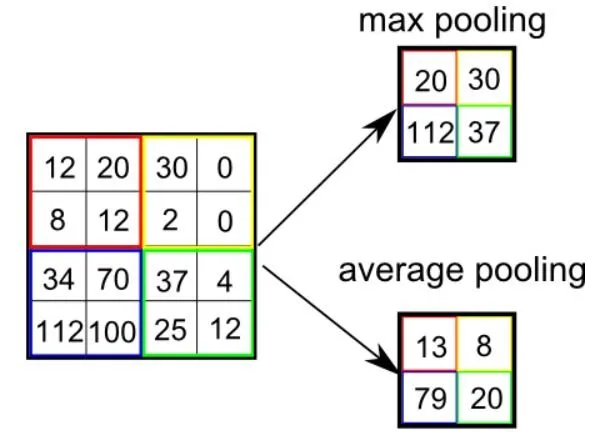
\includegraphics[width=0.5\textwidth]{images/figure12.png}
    \caption{Types of Pooling}
    \label{fig:12}
\end{figure}

\subsection{Mathematical Example of Max Pooling}
Given a $2\times2$ pooling filter applied to a $4\times4$ input will be as below:\\

For an input matrix
$\begin{bmatrix} 1 & 3 & 2 & 1\\ 5 & 6 & 8 & 2\\ 7 & 2 & 9 & 3\\ 4 & 5 & 1 & 0
\end{bmatrix}$, max pooling output matrix will be $\begin{bmatrix} 6 & 8\\ 7 & 9\end{bmatrix}$.

\subsection{Max Pooling v/s Average Pooling}
In addition to dimensionality reduction, Max Pooling also performs as a \textbf{Noise Suppressant} by completely discarding the noisy activations. On the other hand, Average Pooling simply performs dimensionality reduction as a noise-suppressing mechanism. That is why, in general, \textbf{Max Pooling performs a lot better than Average Pooling}. However, the choice between Max Pooling and Average Pooling depends on the specific use case and the nature of the task at hand.\\

In simpler words, \textbf{Max Pooling leads to sparse feature maps but emphasizes the most important activations} (by discarding noise). Since it highlights only the most prominent features (e.g., edges, textures, etc.) that are critical for decision-making, Max Pooling performs better in tasks requiring robustness to noise in input data and preservation of sharp, critical features (e.g., object detection and classification, etc.).\\

On the other hand, \textbf{Average Pooling produces dense feature maps with less emphasis on extreme activations}, but better captures overall patterns by smoothing the outputs by averaging activations. Therefore, if the goal is to generate smooth and generalized (balanced) feature representations and the input data is relatively clean and lacks significant noise, Average Pooling is a better choice.\\

The Convolutional Layer and the Pooling Layer come together and form the i-th layer of a Convolutional Neural Network. Depending on the complexities in the images, the number of such layers may be increased for capturing low-level details even further, but at the cost of more computational power. For example, figure \ref{fig:3} in chapter \ref{chp:1} shows a CNN architecture (to classify handwritten digits from the MNIST dataset) using $2$ Convolutional Layers and $2$ Max Pooling layers one after another.\\

So far we have enabled the model to understand the input image and extract important features (e.g., edges, textures, angles, etc.) in a much simpler matrix form in lower dimensions. Moving on, we will flatten this output and feed it to a regular Neural Network for classification purposes. But before that, we will touch upon another important topic which is important for the Convolutional Layer - \textbf{Activation Functions}.

\section{Activation Functions}
Activation functions in the convolutional layer play a crucial role in Convolutional Neural Networks (CNN). Activation functions introduce non-linearity into the model, enabling it to learn complex patterns and relationships in the data. Without activation functions, the CNN would behave as a linear model, regardless of the number of layers, limiting its ability to solve non-linear problems such as image classification, object detection, and natural language processing.\\

By enabling the network to learn non-linear transformations and hierarchical features, activation functions are essential for the success of deep learning models in solving complex real-world problems.\\

Below are some commonly used activation functions:
\begin{itemize}
    \item \textbf{ReLU (Rectified Linear Unit) function}: It ensures sparsity by retaining only positive activations, which not only introduces non-linearity but also improves computational efficiency and helps avoid the vanishing gradient problem.\cite{nair2010relu}
    \begin{equation}
        \text{ReLU}(z): \mathbb{R} \to \mathbb{R}_{\geq 0}, \quad \text{ReLU}(z) := \max(0, z)
        \label{eqn:5}
    \end{equation}
    \item \textbf{Sigmoid function}: Commonly used in the output layer of a binary classification task, as it maps values to the range $(0, 1)$, representing probabilities. Suitable when the model needs to output probabilities or interpret values as likelihoods, but it can suffer from vanishing gradients.\cite{hochreiter1997lstm, rumelhart1986learning}
    \begin{equation}
        \sigma: \mathbb{R} \to (0,1), \quad \sigma(z) := \frac{1}{1+e^{-z}}
        \label{eqn:6}
    \end{equation}
    \item \textbf{Hyperbolic Tangent (tanh) function}: Preferred in hidden layers when inputs are zero-centered, as it maps the input in the range $(-1, 1)$, which helps faster convergence during training. It has more efficient gradient flow than sigmoid function.
    \begin{equation}
        \text{tanh}: \mathbb{R} \to (-1,1), \quad \text{tanh}(z) := \frac{e^z-e^{-z}}{e^z+e^{-z}}
        \label{eqn:7}
    \end{equation}
    \item \textbf{Hard hyperbolic tangent (hardtanh) function}: Provides a faster approximation of the traditional tanh function, maintaining a balance between non-linearity and computational simplicity.
    \begin{equation}
        \text{hardtanh}(z): \mathbb{R} \to [-1,1], \quad \text{hardtanh}(z) := \max(-1, \min(1,z))
        \label{eqn:8}
    \end{equation}
    \item \textbf{Identity function}: While it does not introduce non-linearity, it is occasionally used in skip connections or output layers when no transformation is needed.
    \begin{equation}
        \text{id}(z): \mathbb{R} \to \mathbb{R}, \quad \text{id}(z) := z
        \label{eqn:9}
    \end{equation}
    \item \textbf{Softmax function}: Typically applied at the output layer for multi-class classification tasks, converting raw scores into normalized probabilities.
    \begin{equation}
        \text{softmax}(z) : \mathbb{R}^n \to \mathbb{R}^n, \quad \text{softmax}(z)_j := \frac{e^{z_j}}{\sum_{j=1}^n e^{z_j}}
        \label{eqn:10}
    \end{equation}
\end{itemize}

Together, these activation functions allow CNNs to learn non-linear transformations, capture intricate data patterns, and perform complex real-world tasks effectively.

\section{Fully Connected Layers}
After the earlier layers of convolution and pooling extract local features from the input data, the output from the last pooling layer is flattened into a column vector. This flattened output is fed into a fully connected layer (FC) to aggregate the learned spatial features for classification purposes.\\

\begin{figure}[h!]
    \centering
    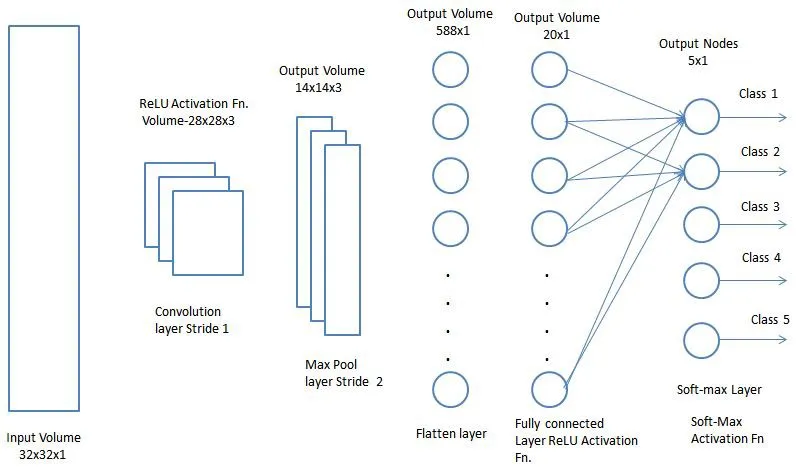
\includegraphics[width=\textwidth]{images/figure13.png}
    \caption{Feeding the flattened final output to regular NN}
    \label{fig:13}
\end{figure}

Fully connected layers play a crucial role in combining the high-level features extracted by the convolutional layers to identify global patterns and relationships. They enable the network to synthesize the extracted features into meaningful representations for decision-making, such as classifying an input image into one of several categories. The addition of fully connected layers is a computationally efficient way to learn non-linear combinations of these high-level features.\\

After the input is flattened and passed through the fully connected layers, backpropagation is performed at each training iteration. Over multiple epochs, the model gradually learns to distinguish between prominent and subtle features in the data. This iterative process enables the network to accurately recognize patterns and classify inputs.\\

In a classification task, the fully connected layer produces a set of values that correspond to the likelihood of the input belonging to each class. These values are converted into probabilities using an activation function like softmax, enabling the network to predict the most probable class for the given input.\cite{krizhevsky2012imagenet}\\

By connecting spatially extracted features to the classification process, fully connected layers act as the final step in converting raw input data into meaningful decisions.

\section{Dropout Layer}
Dropout is a regularization technique to prevent overfitting by randomly "dropping out" (setting to zero) a fraction of neurons' outputs during training.\\

A dropout layer in a Convolutional Neural Network (CNN) uses this technique to force the network to learn redundant, robust features by not relying heavily on specific neurons. The dropout rate, typically between $0.2$ and $0.5$, determines the proportion of neurons to drop. During testing, all neurons are used, and their outputs are scaled by the dropout rate to maintain consistency with training. This helps improve the network's generalization capability on unseen data.\cite{srivastava2014dropout}